% New Chapter %%%%%%%%%%%%%%%%%%%%%%%%%%%%%%%%%%%%%%%%%%%%%%%%
%
\chapter{Proportions, Ratios, and Scaling}\label{chap:proportions}
%
%%%%%%%%%%%%%%%%%%%%%%%%%%%%%%%%%%%%%%%%%%%%%%%%%%%%%%%%%%%%%%

\setcounter{section}{-1}
% New Section %%%%%%%%%%%%%%%%%%%%%%%%%%%%%%%%%%%%%%%%%%%%%%%%
\section{Mathematical Outcome}\label{sec:RatiosOutcome}
%%%%%%%%%%%%%%%%%%%%%%%%%%%%%%%%%%%%%%%%%%%%%%%%%%%%%%%%%%%%%%
The activities of this section are designed to strengthen understanding of fractions and the related concepts of ratios and similarity through applications of proportion, ratio, and scaling. For unit conversion it is assumed the student has a working knowledge of fractions including multiplication and division thereof. The sections on ratios and similarity are presented assuming little to no prior knowledge of the topics.

Through a series of activities mostly focused on things in the world around us such as the moon, peoples' eyes, and the buildings in which we teach and learn, students will
\begin{enumerate}
\item learn to convert units through multiplying fractions
\item work with ratios
\item see the connection between equivalent fractions and equivalent ratios
\item connect proportionality and scale with the world around them
\item calculate heights and weights of large objects by gathering data about smaller ones and using mathematics to extrapolate
\item explore the concept of self-similarity
\end{enumerate}

\newpage
% New Section %%%%%%%%%%%%%%%%%%%%%%%%%%%%%%%%%%%%%%%%%%%%%%%%
\section{Unit Conversion}\label{sec:Conversion}
%%%%%%%%%%%%%%%%%%%%%%%%%%%%%%%%%%%%%%%%%%%%%%%%%%%%%%%%%%%%%%

\subsection{Entrance Activity: One Billion Seconds}
\begin{enumerate}
	\item Write one billion as a numeral (writing its digits, not words). \wbvfill
	\item Convert 5 minutes into seconds. (How many seconds are there in five minutes?) \wbvfill
	\item Convert 240 seconds into minutes. (How many minutes are in 240 seconds?) \wbvfill
	\item Convert 2,022 minutes into seconds. \wbvfill
	\item Convert 2,022 seconds into minutes. \wbvfill
	\item What mathematical operation(s) do you need to do these conversions? ($+,-,\times,\div,\sqrt{\ }$, etc.) \wbvfill
\end{enumerate}

\wbnewpage

%%%%%%%%%%%%%%%%%%%%%%%%%%%%%%%%%%%%%%%%%%%%%%%%%%%%%%%%%%%%%%
\subsection{Activity: One Billion Seconds}
On what day will you (or did you) become one billion seconds old?
\begin{enumerate}
	\item \label{enu:billionsecondsbegin}As we have done before, let's solve a simpler problem first. On what day will you (or did you) become one million seconds old? Write one million as a numeral (writing its digits, not words). \wbvfill
	\item \label{enu:secondsinday}One plan of action is to convert one million seconds into days, and count that many days from your birthday. Not many people know how to convert seconds to days directly, though. We can figure it out!
	\begin{enumerate}
		\item \label{enu:daytohours}Convert one day into hours. \wbvfill
		\item \label{enu:hourstominutes}Convert the number of hours you got in part \ref{enu:daytohours} to minutes. This is how many minutes in one day. \wbvfill
		\item Convert the number of minutes you got in part \ref{enu:hourstominutes} to seconds. This is how many seconds in one day. \wbvfill
	\end{enumerate}
	\item \label{enu:millionsecondsindays}Use your work from question \ref{enu:secondsinday} to convert one million seconds to days. \Instr{ 1,000,000 seconds is about 11.5 days so the complication of leap years is not likely to be an issue.} \wbvfill
	\item \label{enu:birthday}Write down your birthday, including the year. \wbvfill
	\item \label{enu:billionsecondsend}Use your answers to parts \ref{enu:millionsecondsindays} and \ref{enu:birthday} to determine on what day you will become (or became) one million seconds old.\\ \textbf{To think about}: Does it matter what time you were born? \Instr{ Students will hopefully realize that 1,000,000 seconds is neither 11 nor 12 days, and will have to tackle what it means for it to be 11 \textbf{and a half} days. The time of birth will make the difference between one day or the next.} \wbvfill\wbnewpage
	\item Use what you learned from questions \ref{enu:billionsecondsbegin} through \ref{enu:billionsecondsend} to determine on what day you will become (or became) one billion seconds old.\\ \textbf{To think about}: Do all months have the same number of days? Do all years have the same number of days? \Instr{ 1,000,000,000 seconds is exactly $11,574\frac{2}{27}$ days (about 31.7 years). Determining this number exactly should make it easier to figure out how their time of birth affects the answer. Only students born during the last 2/27 of a day (at 10:13:20 PM or later) will need to worry about the time. Some people will undoubtedly have no idea what time they were born, so this issue can be avoided altogether by assuming the birth happened at noon. Students will have to wrestle with how to handle leap years, though. Depending on their birthdate, they will need to account for either 7 or 8 of them. The questions are to make them think twice before trying to calculate the number of seconds in a month or year and using that number as if it were a constant.} \wbvfill\wbnewpage
\end{enumerate}

%%%%%%%%%%%%%%%%%%%%%%%%%%%%%%%%%%%%%%%%%%%%%%%%%%%%%%%%%%%%%%
\subsection{Exit Slip}
\begin{enumerate}
\item How many seconds are there in one year? Does this change from year to year? If so, give all possible answers and explain why there are multiple answers.\wbvfill
\end{enumerate}\wbnewpage

%%%%%%%%%%%%%%%%%%%%%%%%%%%%%%%%%%%%%%%%%%%%%%%%%%%%%%%%%%%%%%
\subsection{Activity: Carats and Carrots}
When you are told the carat weight of a gem stone or piece of jewelry, you are actually being given its mass in carats. A unit of mass you are probably more familiar with is the gram. In fact, $1\text{ gram}=5\text{ carats}$, and we call the number 5 the conversion factor between carats and grams. 
\begin{enumerate}
\item Convert 26 grams to carats. \wbvfill
\item If the mass of an object is written in both carats and grams, which number will be numerically larger---the number of grams or the number of carats? \wbvfill
\item Should you multiply by 5 or divide by 5 to convert a mass in carats to a mass in grams? Why? \Instr{ 1 gram is more mass than 1 carat, so the mass of an object in grams is numerically smaller than its mass measured in grams. Therefore, one should divide mass in carats by 5 to get mass in grams.} \wbvfill
\item What is the mass of a $\frac{1}{4}$-carat diamond in grams? \wbvfill
\item \label{enu:pounds-grams}Given that $1\text{ pound}=453.6\text{ grams}$, how many pounds does a $1$-carat diamond weigh? \wbvfill
\item If you buy a half pound of carrots, how many carats of carrots do you have? Convert first from pounds to grams, and then from grams to carats. \wbvfill
\item If you ordered $2,000$ carats of cheese at the deli, how many pounds would you expect to get (assuming the deli-worker didn't just stand there looking at you funny!)? \wbvfill\wbnewpage
\end{enumerate}

%%%%%%%%%%%%%%%%%%%%%%%%%%%%%%%%%%%%%%%%%%%%%%%%%%%%%%%%%%%%%%
\subsection{Activity: To the Moon!}
NASA's Artemis project is intended to bring people to the surface of the moon as early as 2025. The first Artemis mission was scrubbed on August 29, 2022 and then again on September 3, 2022. The first launch was then rescheduled for mid-October 2022. "With Artemis missions, NASA will land the first woman and first person of color on the Moon, using innovative technologies to explore more of the lunar surface than ever before...We’re going back to the Moon for scientific discovery, economic benefits, and inspiration for a new generation of explorers." (\href{https://www.nasa.gov/specials/artemis/}{Artemis})

\bigskip\noindent\textbf{The Activity:} How far is the moon from Earth?

\smallskip\noindent{}I bet you expected to have to work for that answer. Not this time! On average, the moon is $.00000004063$ light years away . OK, OK, so you'll have to work a little. \Instr{ Students may need some help getting over the fact that even though light years may sound like a measure of time, they are a measure of distance.}
\begin{enumerate}
\item Will the number of miles from Earth to the moon be greater or less than the number of light years? \wbvfill
\item 1,000,000,000,000\text{ miles}=0.170107795023\text{ light years} so dividing one by the other equals a sort of ``one''. Multiplying by either fraction, therefore, leaves distances unchanged! Which fraction should you multiply $.00000004063$ light years by to convert to miles, and why?
\[
\frac{1,000,000,000,000\text{ miles}}{0.170107795023\text{ light years}}\quad\text{or}\quad \frac{0.170107795023\text{ light years}}{1,000,000,000,000\text{ miles}}
\]
\Instr{ Students should explain their choice by noting that they are trying to make the number larger and so need to multiply by a number greater than one, or they should notice that their choice leads to cancelation of light years, or something similar.}\wbvfill
\item Carry out the product as planned.\par\medskip
$.00000004063\text{ light years}\times\frac{\qquad\qquad\qquad\qquad\qquad}{\qquad\qquad\qquad\qquad\qquad}=$\par\medskip
\item Now write that product without the numbers, retaining only the units.\par\medskip
$\text{ light years}\times\frac{\qquad\qquad\qquad\qquad\qquad}{\qquad\qquad\qquad\qquad\qquad}=$\par\medskip
Do the light years cancel?
\item Redo the calculation using the equation 1 light year$=$5,878,625,000,000 miles.\par\medskip
$.00000004063\text{ light years}\times\frac{\qquad\qquad\qquad\qquad\qquad}{\qquad\qquad\qquad\qquad\qquad}=$\par\medskip
Did you get the same answer? \wbnewpage
\end{enumerate}

%%%%%%%%%%%%%%%%%%%%%%%%%%%%%%%%%%%%%%%%%%%%%%%%%%%%%%%%%%%%%%
\subsection{Exit Slip}
\begin{enumerate}
\item Convert the average distance between the sun and Earth, 93 million miles, into light years.\wbvfill
\item A typical tire pressure for automobiles is 220 kPa (kilopascals). Use the fact that 1.25 kPa equals 0.1813 psi (pounds per square inch) to convert typical tire pressure to psi. Source: \href{https://www.pirelli.com/tires/en-us/car/driving-and-tire-tips/how-to-read/recommended-tire-pressure}{Pirelli}.\wbvfill
\item Prior to 1896, the length of the Kentucky Derby was 12 furlongs. Source: \href{https://www.kentuckyderby.com/history/kentucky-derby-history}{KentuckyDerby.com}. Use the fact that one furlong equals one eighth of a mile to convert the original length of the Kentucky Derby to miles.\wbvfill
\item Using the facts that (a) one furlong equals one eighth of a mile and (b) there are 5280 feet in one mile, what is the conversion factor between feet and furlongs?\wbvfill
\end{enumerate}\wbnewpage
%%%%%%%%%%%%%%%%%%%%%%%%%%%%%%%%%%%%%%%%%%%%%%%%%%%%%%%%%%%%%%


\iffalse

% New Section %%%%%%%%%%%%%%%%%%%%%%%%%%%%%%%%%%%%%%%%%%%%%%%%
\section{Density}\label{sec:proportions}
%%%%%%%%%%%%%%%%%%%%%%%%%%%%%%%%%%%%%%%%%%%%%%%%%%%%%%%%%%%%%%

You're on a family vacation, and your parents get the idea to bring everyone to the nearby odditorium. You're not sure it will be any fun, but your parents are insistent and your sibling thinks it's a great idea. It turns out the things at the odditorium are truly odd. There's the world's smallest automobile, authentic shrunken heads, and sculptures made from recyclables. There's also this mannequin of the world's tallest person next to a young lady clearly enjoying the place. You spy the same young lady just outside the odditorium with this humongous marble.
\begin{center}
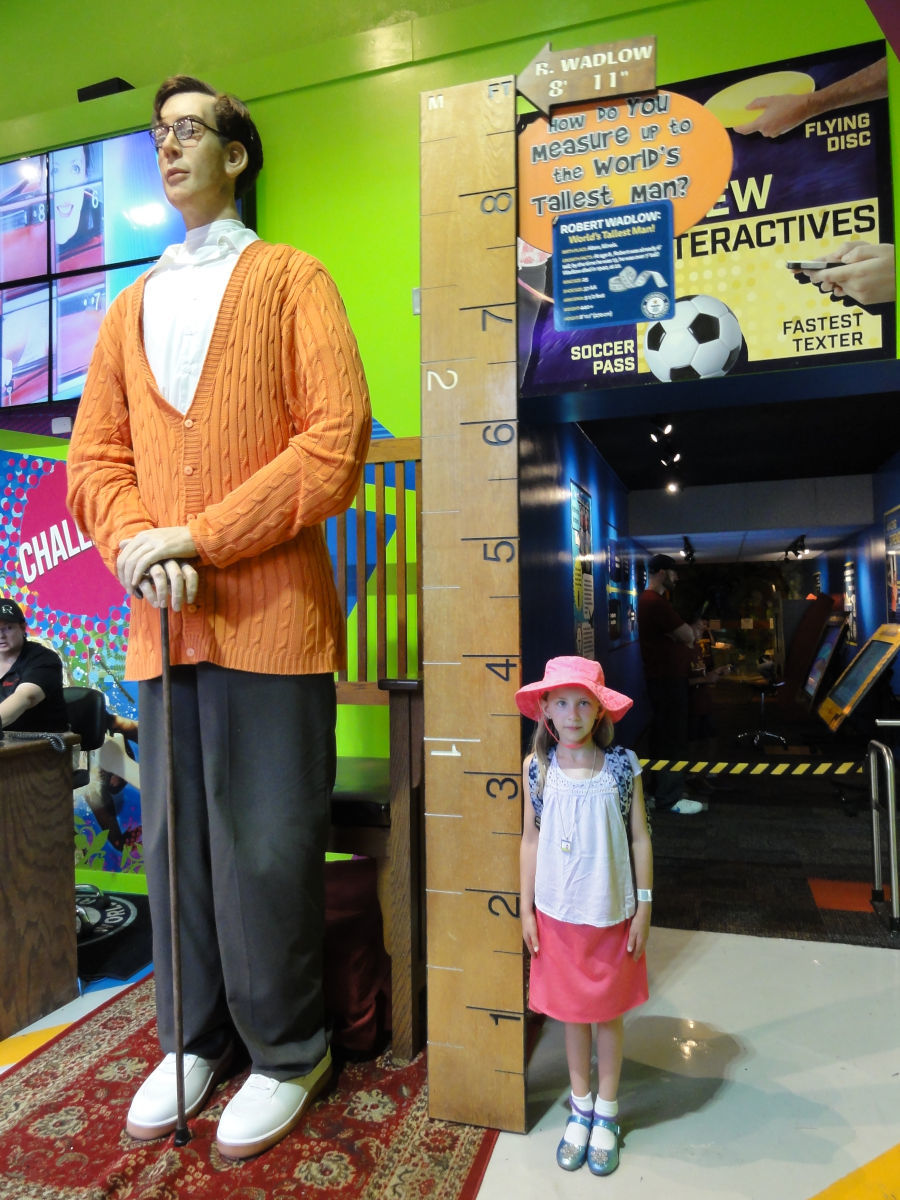
\includegraphics{images/OdditoriumTallMan} 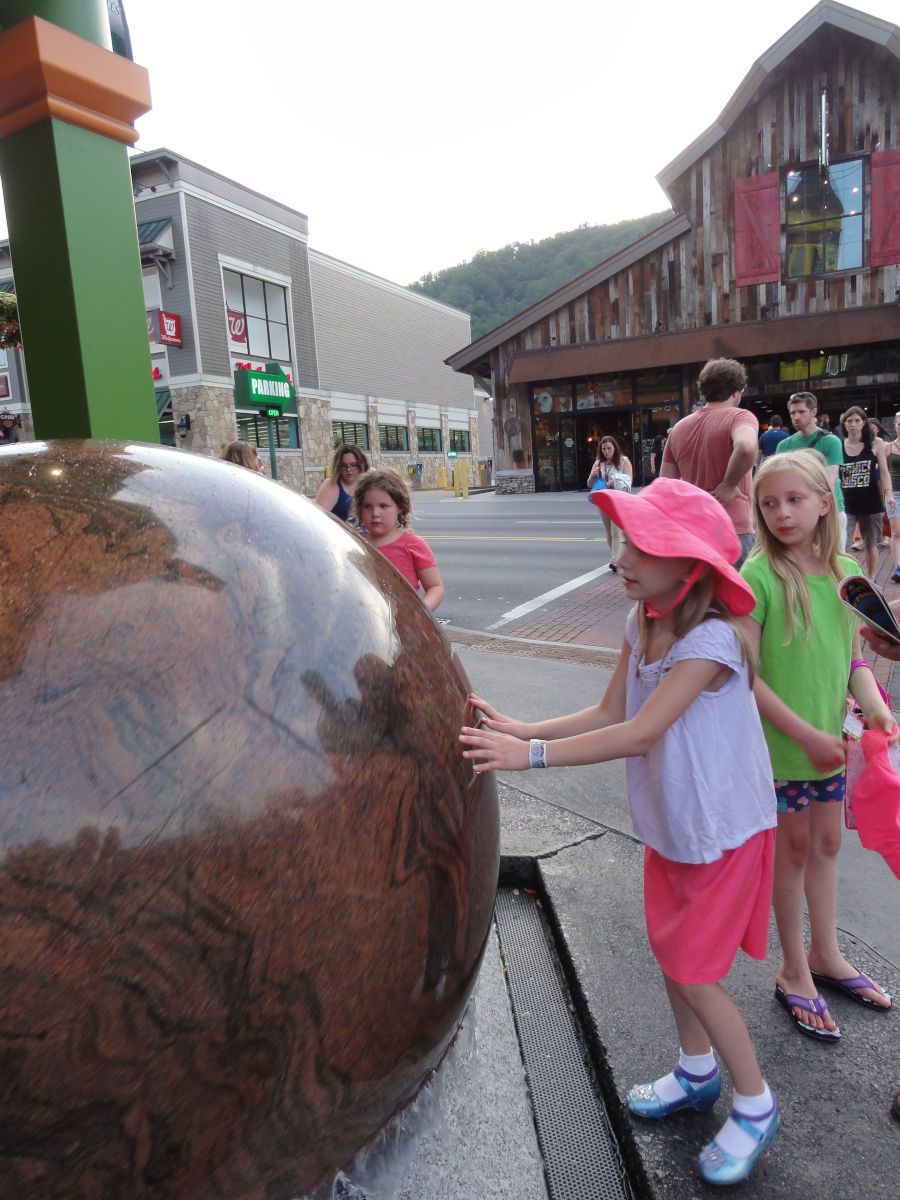
\includegraphics{images/OdditoriumSphereWithYouth}
\par\end{center}

Curiously, she is spinning the marble all by herself! The sign nearby notes that the sphere ``is floating on 1/254 inches of water and can easily be stopped and spun in another direction---try it!'' You think to yourself, ``that ball looks really heavy. Just how much weight is she pushing around?''

Preparation (to be done at home before class) Gather several stones, each one about the size of a walnut. Put them somewhere so you won't forget to bring them to class!\bigskip{}

\Instr{ 
\begin{act}Mystery Bags\end{act}
Preparation: Before the lesson, fill two large brown paper bags with light-weight materials, such as Styrofoam, cotton, shredded tissue paper, etc. Fill two large brown paper bags with heavy-weight materials, such as container filled with rocks, cans of paint, heavy metal objects, etc. Close the bags and number each bag. Make the exterior of the bags look the same. In class
\begin{enumerate}
\item Place the four bags next to each other on a table.
\item Ask the students if they can tell anything about how heavy each bag is by mere observation.
\item Ask them to predict the relative weights of the four bags.
\item Next, have one member of each group come up and pick up each of the bags and arrange the bags in descending order of mass.
\item Discuss with students the fact that although the bags looked very similar and seemed to occupy the same amount of space (volume), they had different masses. Explain that volume is how much space something takes up.
\end{enumerate}

\begin{act}The Soda Cans are Different?\end{act}
\begin{enumerate}
\item Hold up two cans of soda, one diet and one regular. Ask students if they weigh the same and how they know. Check for understanding: If students say they weigh the same because they're the same size, remind them of what they learned in the previous activity. 
\item Give students a balance and two sodas for each group (diet and regular). Let them measure the mass of each. Discuss with students that the cans have the same volume, but the mass of each is different. Let them share their ideas about why the masses are different. Students may focus on the difference in ingredients between the two sodas without relating it to the mass of the sodas. Be sure to focus students on the concepts of mass, volume, and density before giving the following assignment.
\item When students are finished, present them with the following scenario: The Coca-Cola Company has been getting angry letters from drinkers of Diet Coke. Because their soda weighs less they feel like they're getting ripped off. If they pay the same amount for a diet coke it should have the same amount of soda in it. It is your job as manager of customer relations to answer these angry letters. For homework write a sample letter to be approved by the company president that contains the following: A scientific explanation of why the Diet Coke weighs less, and a sentence or two addressing the customers' concerns that they are getting less soda than in a regular can or bottle. Then, write a memo to the president of the company in which you outline at least one solution the company can do to fix this problem and make customers happy. Remember -- your next promotion depends on how well you solve problems for the company!
\end{enumerate}
} % end \inst

\begin{act}Searching the Classroom\end{act}
\Instr{  Students will connect the idea of how comparing the magnitudes of fractions with the idea of density. To facilitate the discussion, have them solve and discuss the following problems.}
\begin{enumerate}
\item \label{en:samedenominator}Arrange the fractions in order of increasing size.
\begin{enumerate}
\item $\frac{28}{101}$, $\frac{15}{101}$, $\frac{86}{101}$, $\frac{76}{101}$
\item $\frac{74}{101}$, $\frac{40}{101}$, $\frac{4}{101}$, $\frac{62}{101}$
\end{enumerate}
\item Explain how you solved the problem in question \ref{en:samedenominator}. What made it easier than it could have been?
\item \label{en:samenumerator}Arrange the fractions in order of increasing size.
\begin{enumerate}
\item $\frac{11}{37}$, $\frac{11}{55}$, $\frac{11}{47}$, $\frac{11}{49}$
\item $\frac{11}{92}$, $\frac{11}{16}$, $\frac{11}{47}$, $\frac{11}{67}$
\end{enumerate}
\item Explain how you solved the problem in question \ref{en:samenumerator}. What made it easier than it could have been?
\item \label{en:nosame}Arrange the fractions in order of increasing size.
\begin{enumerate}
\item $\frac{1}{10}$, $\frac{9}{4}$, $\frac{3}{5}$, $\frac{8}{3}$
\item $\frac{86}{75}$, $\frac{7}{33}$, $\frac{89}{83}$, $\frac{22}{41}$
\end{enumerate}
\item Explain how you solved the problem in question \ref{en:nosame}. What made it more difficult than the others? What strategies were you able to use to facilitate the task? \Instr{  Some students may simply convert each fraction to a decimal value for purpose of ordering. Some students may rewrite all fractions in a list with the same denominator (or numerator if they have taken a clue from the previous exercises). Still others may notice that in each question two of the fractions are greater than 1 and two are less than 1. They only need to compare the two pairs to complete the ordering, and that part can be done by approximation: $\frac{22}{41}\approx\frac{1}{2}$ while $\frac{7}{33}<\frac{1}{4}$ for example.}
\end{enumerate}
\Instr{  Students should now know that objects can have the same volume but different masses. Now students will explore objects that have identical masses but different volumes.}
\par
\noindent Find two different objects in the room with the same masses. They can not be two identical items. Record your finding in your notebook.
\par
\Instr{  
\begin{enumerate}
\item Once each group is finished allow them to present their findings and discuss the rationale for the items that they tried using the information from their findings.
\item Discuss with the class that some items have the same masses, but take up more or less space (volume). Some items take up the same amount of space (volume) but have more or less mass. A way to talk about the relationship between mass and volume is density, measured in mass per unit volume.
\item Discuss the fact that a fraction with a greater numerator is greater than a fraction with a smaller numerator provided the denominators are the same. Relate this to the formula for density (density=mass/volume), so the object with the greater mass (numerator) has greater density provided they occupy the same volume (denominator).
\item Discuss the fact that a fraction with a lesser denominator is greater than a fraction with a greater denominator provided the numerators are the same. Relate this to the formula for density (density=mass/volume), so the object with the lesser volume (denominator) has greater density provided they have the same mass (numerator).
\end{enumerate}
}

\begin{act}Cubic Densities\end{act}
\Instr{  Present students with 4 cubes of the same size but made of different materials.}
\par
\begin{enumerate}
\item Predict the order of density of the four cubes, greatest to smallest and record your predictions. \Instr{  Ask students to share their predictions.}
\item Weigh each cube in grams using the scale.
\item Measure the dimensions of the cubes to the nearest cm. 
\item Find the volume of each cube in cubic cm.
\item Divide the mass of the cube by its volume to determine its density in grams per cubic centimeter. Record results in your notebook.
\item Compare your calculations to your predictions.
\end{enumerate}

\begin{act}Centimeter Cubes and Soda Cans\end{act}
\Instr{  Students will need to understand the ideas of percent difference and percent error. Use these exercises to facilitate the discussion/learning.}
Percent difference, percent error, percent change, and any other use of percentages involve two understood, implied, or explicitly stated quantities, a comparison value, and a reference value to which the comparison value is compared. For example, at a 10\% off sale, the reference value is the regular price. For each item, the discount is calculated as 10\% of this reference value, and is therefore a comparison value as it is 10\% comapared to the reference value. The discount is then taken, resulting in a price that is 10\% lower than the regular price. There is thus a 10\% difference between the regular price and the sale price, \textit{\textbf{but only if we understand that the regular price is the reference price! We get different results if we use the sale price as the reference for computing the 10\%.}} The following exercises will guide you through an exploration of these ideas. In general, you should use the conceptual formula \[\text{percentage}=\frac{\text{comparison value}}{\text{reference value}}\times 100\%\]
\begin{enumerate}
\item Compute a percentage from the given comparison value and reference value.
\begin{enumerate}
\item comparison: $4$; reference: $12$
\item comparison: $12$; reference: $4$
\item comparison: $42$ gallons; reference: $83$ gallons
\item comparison: $2.6$ inches; reference: $32$ inches
\end{enumerate}
\item \label{en:percentExamples}In the following scenario, identify the comparison value and the reference value.
\begin{enumerate}
\item The sale price of an item is \$19.24 while its regular price is \$26. \Instr{  the regular price is the reference value}
\item A chemist is increasing the amount of HCl in a mixture from 3 mL to 4 mL. \Instr{  the original amount is the reference value}
\item A homeowner intends to decrease their monthly energy consumption, which is usually around 530 kWh (kilowatt hours), to 500 kWh. \Instr{  the usual consumption is the reference value}
\end{enumerate}
\item \label{en:percentof}For each example in question \ref{en:percentExamples} what percentage of the reference value is the comparison value? \Instr{  74\%, 133\%, 94.34\%}
\item \label{en:percentdiff}For each example in question \ref{en:percentExamples} calculate the percent difference between the reference and comparison values. Answer using positive percentages and the word "increase" or "decrease", as in "51\% increase" or "32\% decrease". \Instr{  26\% decrease, 33\% increase, 5.66\% decrease}
\item Draw a connection between your answers to questions \ref{en:percentof} and \ref{en:percentdiff}. Explain why the connection you have spotted must be true. \Instr{  Students should surmise that the percentage in \ref{en:percentof} differs from 100\% by exactly the percentage increase or decrease (since the comparison value plus or minus the difference must equal the reference. In other words, it must be 100\% of the reference).}
\item Calculate the percent error of the approximation (as a positive value).
\begin{enumerate}
\item The actual number of students at a high school is 1172 and is estimated at 1200. \Instr{  2.333\%}
\item The actual length of a Subaru Outback is 191.3 inches \href{https://www.carindigo.com/subaru/outback/dimensions}{Carindigo} and is estimated at 15 feet. \Instr{  This is a good time to discuss the fact that percentages are unitless measurements. The numerator and denominator of the conceptual formula must have the same units for the units to "cancel". In this question, the student must convert both measurements to the same unit of measure before subtracting or dividing. 5.907\%}
\end{enumerate}
\item Find the percent difference between the two quantities (i) using the lesser of the two numbers as the reference value; and (ii) using the greater of the two numbers as the reference value.
\begin{enumerate}
\item 90 and 100 \Instr{  11.11\% and 10\%}
\item 30 inches and 40 inches \Instr{  33.33\% and 25\%}
\end{enumerate}
\item Comment on the importance of knowing which quantity is the reference value in a percentage computation.
\end{enumerate}
\Instr{  This works best if students do not yet know that $1\text{cm}^{3}=1\text{mL}$. If they know this, you can use a Sharpie or masking tape to cover the volume written on the can. Some cans should contain diet soda and some not. The soda cans will be used again later so don't let the students drink the soda! Give each group a full soda can and a handful of centimeter cubes.} 
\begin{enumerate}
\item Using the centimeter cubes given to you as a reference, estimate the number of centimeter cubes that would fit into the soda can if they were able to mold to the shape of the can. \Instr{  You might need to encourage them to imagine using clay centimeter cubes that can actually be molded.}
\item What is the volume of that many centimeter cubes? \Instr{  Students need to realize that each centimeter cube is one cubic centimeter in volume, and therefore $n$ centimeter cubes has volume $n$ cubic centimeters.}
\item Your instructor will tell you the actual volume of the can. Compare it to the volume of the estimated number of cubes. Did you underestimate? Overestimate? By what percent was your estimate off? \Instr{  After students have written down their estimates, reveal the volume of the can (have them read it off the can). Have them convert this measurement to cubic centimeters (number of centimeter cubes). Using a web search is acceptable.}
\end{enumerate}

\begin{act}Volume Formulas\end{act}
\begin{enumerate}
\item Calculate the volumes of some spheres. Use the formula $V=\frac{4}{3}\pi r^{3}$.
The first one is done for you.
\begin{center}
\begin{tabular}{|>{\centering}p{0.9in}|>{\centering}p{0.9in}|>{\centering}p{0.9in}|>{\centering}p{0.9in}|}
\hline 
radius & units & volume & units\tabularnewline
\hline 
\hline 
2 & ft. & $\frac{4}{3}\pi(2)^{3}\approx33.51$ & ft.$^{3}$ (cu. ft.)\tabularnewline
\hline 
3 & ft. &  & \tabularnewline
\hline 
4 & ft. &  & \tabularnewline
\hline 
5 & ft. &  & \tabularnewline
\hline 
\end{tabular}
\par\end{center}
\item Calculate the volumes of some cylinders. Use the formula $V=\pi r^{2}h$.
The first one is done for you.
\begin{center}
\begin{tabular}{|>{\centering}p{0.9in}|>{\centering}p{0.9in}|>{\centering}p{0.9in}|>{\centering}p{0.9in}|}
\hline 
radius & height & volume & units\tabularnewline
\hline 
\hline 
2 in. & 3 in. & $\pi(2)^{3}\cdot3\approx37.7$ & in.$^{3}$\tabularnewline
\hline 
14 in. & 21 in. &  & \tabularnewline
\hline 
4 in. & 3 in. &  & \tabularnewline
\hline 
10 in. & 3 in. &  & \tabularnewline
\hline 
\end{tabular}
\par\end{center}
\end{enumerate}

\subsection*{Exercises}
\begin{enumerate}
\item Calculate the volumes of some regular tetrahedra. Use the formula $V=\frac{s^3}{6\sqrt2}$ where $s$ is the length of a side.
The first one is done for you.
\begin{center}
\begin{tabular}{|>{\centering}p{0.9in}|>{\centering}p{0.9in}|>{\centering}p{0.9in}|>{\centering}p{0.9in}|}
\hline 
side & units & volume & units\tabularnewline
\hline 
\hline 
2 & ft. & $\frac{2^3}{6\sqrt2}\approx0.9428$ & ft.$^{3}$ (cu ft)\tabularnewline
\hline 
3 & ft. &  & \tabularnewline
\hline 
4 & ft. &  & \tabularnewline
\hline 
5 & ft. &  & \tabularnewline
\hline 
\end{tabular}
\par\end{center}
\item Calculate the volumes of some pyramids. Use the formula $V=\frac{1}{3}Bh$ where $h$ is the height and $B$ is the area of the base.
The first one is done for you.
\begin{center}
\begin{tabular}{|>{\centering}p{0.9in}|>{\centering}p{0.9in}|>{\centering}p{0.9in}|>{\centering}p{0.9in}|}
\hline 
base & height & volume & units\tabularnewline
\hline 
\hline 
square with 2 in. sides & 3 in. & $(2\cdot 2)\cdot3=12$ & in$^{3}$\tabularnewline
\hline 
triangle with base 5 in. and height 7 in. & 21 in. &  & \tabularnewline
\hline 
circle with radius 4 in. & 3 in. &  & \tabularnewline
\hline 
\end{tabular}
\par\end{center}
\end{enumerate}

\begin{act}Calculating v. Measuring Volume\end{act}
\Instr{  Give each group of students a metal dowel, a graduated cylinder, water, and a centimeter ruler.}
\par
\begin{enumerate}
\item Calculate the volume of the dowel.
\begin{enumerate}
\item Measure the circumference of the small metal dowel. \Instr{  It may be helpful to wrap a strip of paper around the dowel and mark one circumference. The paper can then be laid flat and the distance from end to the mark measured.}
\item Measure the length of the dowel.
\item Use the formula for a cylinder to calculate its volume. \Instr{  Students will need to modify the formula or calculate the radius from the circumference first.}
\item Measure the inner circumference of a graduated cylinder. \Instr{  Again, a strip of paper should be used for this measurement.}
\item Measure the distance from the bottom of the cylinder to the topmost graduation.
\item Calculate the volume of liquid that the cylinder would hold if filled to that line.
\item Compare your calculation to the marking on the cylinder. Do the volumes agree? How do you explain any discrepancy? \Instr{  Neither the markings nor any measurement is perfectly accurate, so the two volumes will likely disagree by a small amount---hopefully less than 10\%.}
\item Calculate the percent difference between the calculated and marked volumes.
\end{enumerate}
\item Measure the volume of the metal dowel.
\begin{enumerate}
\item Fill the graduated cylinder with water to a convenient level (one of the graduations) about 3/4 full. Record the volume of water.
\item Put the metal dowel in the graduated cylinder making sure it is entirely submerged. Read the volume on the graduated cylinder again.
\item According to this experiment, what is the volume of the dowel? Explain. \Instr{  Students may need some guidance calculating and explaining. Mathematically, the first reading is the volume of water in the cylinder. The second reading is the volume of water + the volume of the dowel. The volume of the dowel is therefore the difference between the first and second readings (volume of water + volume of dowel) - (volume of water).}
\item Compare the measured volume of the dowel with the calculated volume of the dowel by calculating the percent difference. Do the volumes agree? How do you explain any discrepancy? \Instr{  Neither the markings nor any measurement is perfectly accurate, so the two volumes will likely disagree by a small amount---hopefully less than 10\%.
\item Review the concept of determining volume by displacement of water with all students.
\item Compare and contrast the calculating and measuring of the volume of the dowel.
}
\end{enumerate}
\end{enumerate}

\begin{act}Liquid Density\end{act}
\Instr{  Preparation: Gather several liquids of varying density: for example, isopropyl alcohol, glycerin, water, soda, epsom salt solution, kosher salt solution, sugar solution. Use food coloring, if desired, to make the density differences more visual. Be sure to try your own test of this simulation to get the correct density numbers using your lab equipment. The number of stations can be adjusted depending on the size of the class and number of stations desired.}
\par
\begin{enumerate}
\item \Instr{  Display an unshaken bottle of Italian salad dressing or homemade concoction of oil and vinegar or oil and water.} Why are the fluids in different layers. \Instr{  Discuss immiscibility (oil and water don't mix) and guide students toward observation that fluids are in layers because one is more or less dense than another, meaning that the ratio of its mass to volume is different.}
\item \Instr{  Shake the bottle.} Draw or describe the settling process of the shaken bottle. \Instr{   \textquotedblleft The fluids settled back into layers because the densities of the liquids are not the same. The one at the top is less dense than those below it. The density of the bottom layer is greater.\textquotedblright{} for example}
\item At your station, measure 100 ml of the liquid. Pour the liquid into the empty plastic cup on the balance that has been zeroed for the weight of the cup. Record the mass of the liquid. Rinse the cup and dry. 
\item Repeat the procedure at each liquid station. 
\item Calculate the density of each liquid. \Instr{  To determine the density of each liquid in grams per ml, divide mass of liquid by 100 because the volume of liquid was 100 ml.} 
\Instr{  \item Plot densities of each liquid on a bar graph on classroom computer using a spreadsheet.}
\item Predict the order into which the liquids would settle if they were all added to a clear bottle (and were mutually immiscible). Draw or describe the order in your notebook.
\Instr{  \item If liquids have been colored with food coloring, add 10 ml of each liquid except for the water to a soda bottle and observe the results.}
\end{enumerate}

\subsection*{Exercises}
\begin{enumerate}
\item Research and record the densities of gasoline, diesel fuel, and mercury.
\item Research and record the densities of as many of the following liquids as you can find: cow's milk, honey, tar, seltzer, melted cheese.
\item Research and record the densities of at least two liquids different from any in these exercises or from any class discussions.
\end{enumerate}

\Instr{ 
\begin{act}Review\end{act}
\par
Review what is now known about density. 
\begin{packedItem}
\item Density is a measurement of the compactness of an object.
\item Density is a property that is determined by the ratio of a substance's mass to its volume.
\item Less dense objects will rise above objects with a greater density.
\item Denser objects will fall below objects with less density.
\end{packedItem}
}

\begin{act}Explain in Your Own Words\end{act}
\begin{enumerate}
\item Explain why the metal dowel sank in the water using
the word ``dense'' or ``density''.
\end{enumerate}

\subsection*{Exercises}
\begin{enumerate}
\item Research and record the densities of three solid materials known to float in pure water.
\item \label{en:sink}Research and record the densities of three solid materials known to sink in pure water.
\item Research and record the density of the water in the Dead Sea, which is very heavily salted.
\item Would any of the materials that sink in pure water (from question \ref{en:sink}) float in the Dead Sea? Explain how you know.
\end{enumerate}

\begin{act}Sink or Float\end{act}
\begin{enumerate}
\item Retrieve the masses and volumes of the soda cans from your notes (one diet, one not). 
\item Predict whether the cans will sink or float in water. \Instr{  Coax the fact that the density of water would be a VERY helpful point of information out of the students. Once they have made this observation, remind students that water has a density of 1 g/cc. If that fact has not been covered, allow them to discover it by experiment and/or web search.}
\Instr{  \item After predictions are made, put the two cans in water to test. You may want to test this ahead of time, too, to make sure one can sinks while the other floats. You might have two buckets of water--one with salt water strong enough to float both cans, and one with plain water--to prompt a discussion of what is going on.}
\end{enumerate}

\begin{act}Some Predictions\end{act}
\begin{enumerate}
\item Measure the densities of the walnut size stones you have collected. \Instr{  Students should know how to do this by measuring their volumes (displacement of water in a graduated cylinder) and masses and dividing the two.}
\item Have students estimate the volume of the giant marble from the picture with the young lady. \Instr{  They may need to wrestle with unit conversion. They might need a reminder of the volume of a sphere formula (activity 6). Give them time and encouragement to work this out themselves.}
\item Have students use this information to predict the mass of the marble. \Instr{  They may need some prompting to understand that the densities of the stones they calculate can be used as estimates of the density of the giant marble, under the assumption that they are made of the same, or similarly dense, material. They should be able to figure out for themselves that the product of the numbers from parts 1 and 2 give an answer. You may wish to discuss unit analysis if it has not been discussed yet: $\text{volume}\cdot\frac{\text{mass}}{\text{volume}}=\text{mass}$. You may instead, or in addition, choose to have them simply rationalize this calculation: ``If a marble weighs 2 grams per cubic centimeter and the marble is 100 cubic centimeters in volume, it must have a mass of 200 grams'' (2 grams for every cubic centimeter). The sign in the background of this \href{https://upload.wikimedia.org/wikipedia/commons/5/5b/5-ton_floating_granite_ball.jpg}{wikimedia photo} gives the mass. The marble is in front of the Ripley's Believe it or Not! odditorium in Gatlinburg, TN. They can visit it in real life!
\item Have the groups present their estimates to the class. You may want to offer a prize to the group who gets the closest (they get to take the sodas home with them?).}
\end{enumerate}

\begin{act}X-ray Vision?\end{act}
\noindent Give or show students a softball and a baseball with the same type of covering.
\par
\begin{enumerate}
\item Do you think the inside (what's under the cover)
is the same material or different in the two balls?
\item Support your assertion with some data. \Instr{  Hopefully they will think to measure their densities---different densities means different materials (or at least different levels of compaction of the same material, like two balls of yarn, one that is wound tighter than the other). Have at least one group present their supporting reasons to the class.}
\end{enumerate}

\fi

\wbnewpage
% New Section %%%%%%%%%%%%%%%%%%%%%%%%%%%%%%%%%%%%%%%%%%%%%%%%
\section{Proportions and Ratios}\label{sec:Ratios}
%%%%%%%%%%%%%%%%%%%%%%%%%%%%%%%%%%%%%%%%%%%%%%%%%%%%%%%%%%%%%%

\subsection{Entrance Activity: Rice}
You've been following the directions on the bag of rice you recently purchased at the grocery store.
\begin{center}
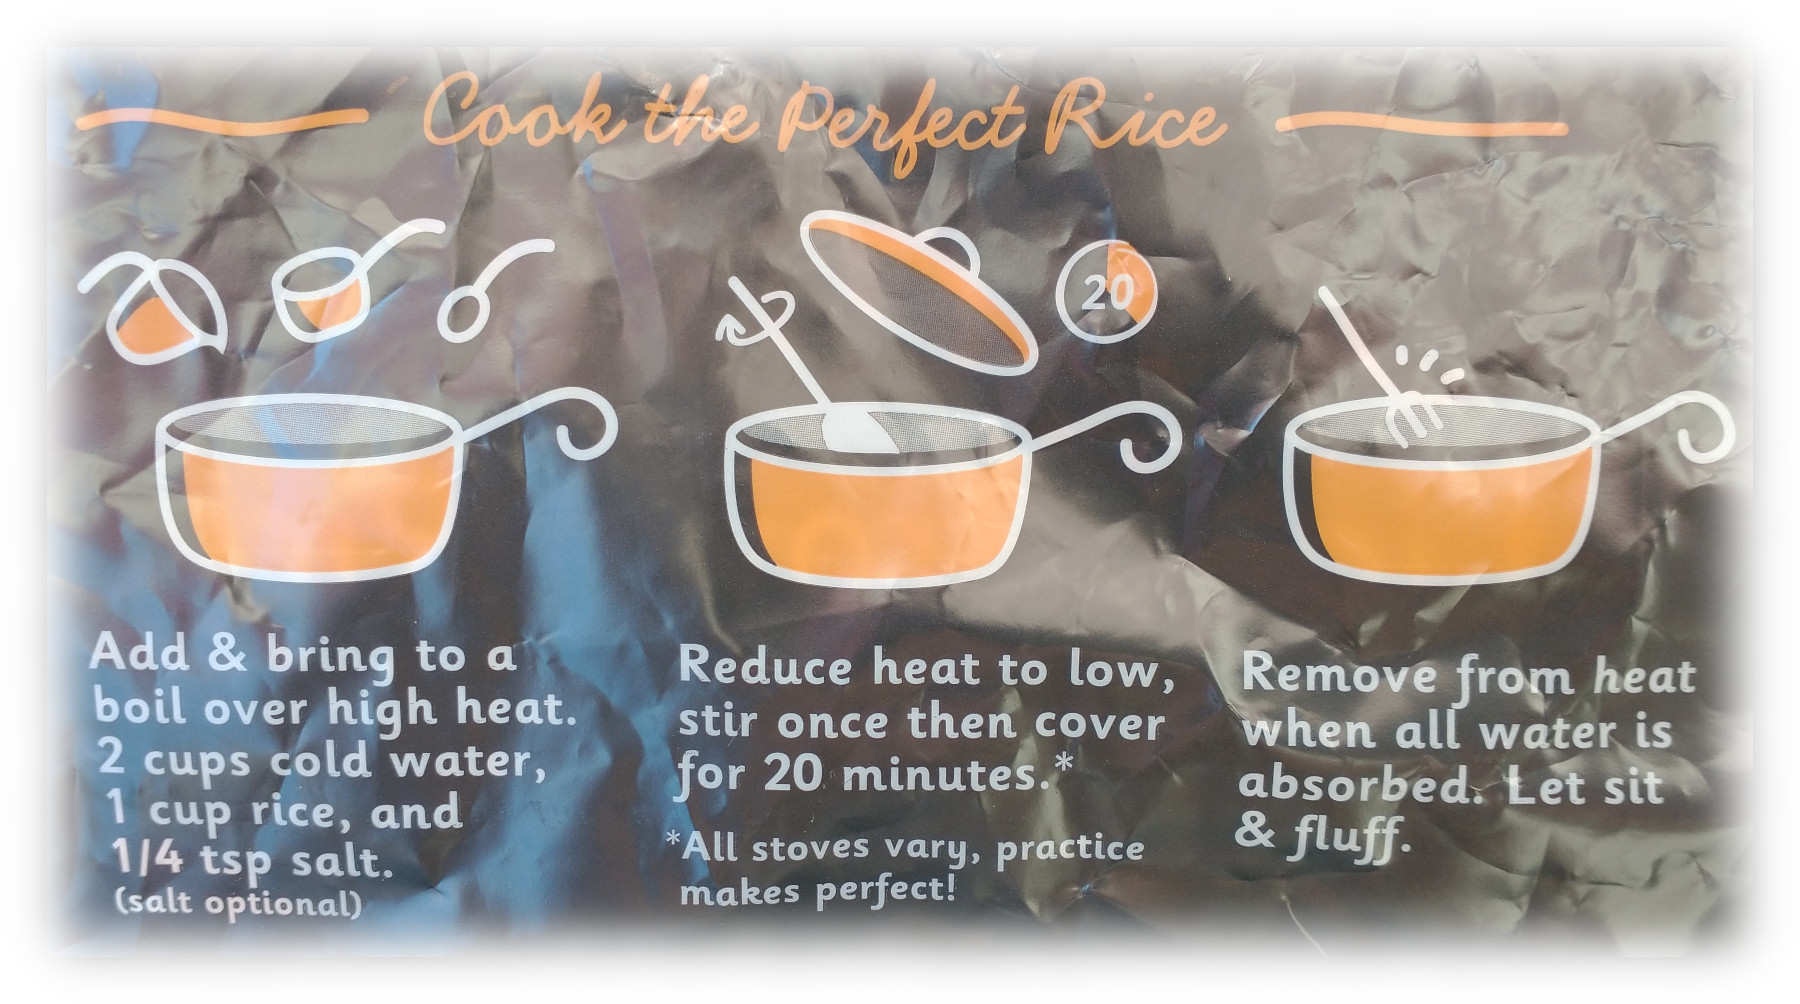
\includegraphics[width=5in]{images/RiceBag}
\par\end{center}
Every time you make the rice, you do it according to the directions---2 cups of water, 1 cup of rice---but it just makes too much! About one third of it is always left over. Learning from this experience, you decide you will use only 2/3 cups of rice. But how much water should you use? Still 2 cups? No. The directions on the bag have you using twice as much water as rice, so you should continue to use twice as much water as rice! For 2/3 cups of rice, you should use $2\cdot(2/3)=4/3$, or $1\frac13$, cups of water. If you used 2 cups of water with 2/3 cups of rice, the water and rice would be out of proportion. You would be using 3 times as much water as rice!
\begin{enumerate}
\item You're having guests and need to cook two cups of rice. How much water should you use?\wbvfill
\item A recipe for rice pudding asks that you start by cooking 3/4 cups of (uncooked) white rice according to package directions. You still have that much rice left in your package. How much water will you need to use?\wbvfill
\item How much rice can you cook with 3 cups of water?\\\Instr{  Students are likely to simply double the 3 since that's what they had to do in the first two questions. Attentive students will notice they've been given an amount of water rather than rice, so they need to have the 3. The amount of water still needs to be twice that of rice, so $1\frac12$ cups.}\wbvfill
\end{enumerate}

\wbnewpage
\subsection{Activity: Ratios and the Colon Notation}
\begin{enumerate}
\item The proper way to cook any amount of rice from the bag in the entrance activity is to use twice as much water as rice. The volumes of water and rice used in cooking should stay in proportion. We might also say that to cook the rice we maintain a 2 to 1 water-to-rice \textbf{ratio}. The symbol used for ratios is the colon. Fill in the blanks to see the water-to-rice ratio written using the colon notation.
\begin{center}
\begin{tabular}{ccc}
 & : & \tabularnewline
\cline{1-1} \cline{3-3} 
amount of water &  & amount of rice\tabularnewline
\end{tabular}
\end{center}
\item In a baseball game where the score is 9 to 6, the announcer might say the winning team is outscoring their opponent 3-to-2, meaning that the winning team is scoring 3 points for every 2 points scored by the losing team. Write the ratio 3-to-2 using colon notation.\wbvfill
\item In a large high school auditorium, the girls outnumber the boys 5-to-4, meaning for every 5 girls there are only 4 boys. Write the ratio 5-to-4 using colon notation.\wbvfill
\item Fill in the blanks in the table where the winning team is outscoring their opponent by a 3:2 ratio.
\begin{center}
\setlength{\extrarowheight}{12pt}
\begin{tabular}{l|>{\centering}p{0.5in}|>{\centering}p{0.5in}|>{\centering}p{0.5in}|>{\centering}p{0.5in}|>{\centering}p{0.5in}}
winning team score & 3 & 6 & 9 & 12 & 15\tabularnewline
\hline 
losing team score &  &  & 6 &  & \tabularnewline
\end{tabular}
\end{center}
\item Fill in the blanks in the table where  girls outnumber boys 5:4.
\begin{center}
\begin{tabular}{l|>{\centering}p{0.75in}|>{\centering}p{0.75in}|>{\centering}p{0.75in}|>{\centering}p{0.75in}}
girls & 100 &  & 195 & \tabularnewline
\hline 
boys &  & 124 &  & 200 \tabularnewline
\end{tabular}
\end{center}
\end{enumerate}
\setlength{\extrarowheight}{0pt}

\wbnewpage
\subsection{Activity: Body Mass Index}
In a 2012 \href{https://www.medicalnewstoday.com/articles/245328#1}{MedicalNewsToday article}, research suggests that waist-to-height ratio is a better predictor of health problems such as high blood pressure, diabetes, heart attacks, and strokes than is BMI (Body Mass Index).
\begin{enumerate}
\item A $5\frac12$ foot tall person with a 32 inch waist has what waist-to-height ratio?\wbvfill
\item According to the article, keeping your waist-to-height ratio at 0.5:1 or lower can increase your life expectancy. A 6 foot tall person should keep their waistline how small to increase their life expectancy?\wbvfill
\end{enumerate}

\subsection{Activity: One Blue, Seven Brown}
\begin{enumerate}
\item What is the ratio between the number of students in this class with brown eyes to that of students with other colored eyes?\wbvfill
\item If the University has 9,127 students, and the ratio of brown-eyed students to non-brown-eyed students matches that in this classroom, how many brown-eyed students are there in total? \wbvfill
\item Repeat the exercise, but now catalog students as having blue eyes, brown eyes, or neither (somewhere in between). The person with the bluest eyes in the classroom has blue eyes. \Instr{  This should start a discussion of what it means to talk about the ratio among three different measurements. Encourage them to eventually think in terms of a blue:brown:neither ratio. Discuss how this makes ratios and fractions different.}\wbvfill\wbvfill
\end{enumerate}

\wbnewpage
\subsection{Activity: Equivalent Ratios}
\begin{enumerate}
\item There are 2.54 centimeters in an inch. That means there is a 2.54:1 ratio between its length measured in centimeters and its length measured in inches. How many centimeters are there in one foot (12 inches)?\wbvfill
\item It is also true that the ratio between a length measured in centimeters and a length measured in inches is 127:50. Use this ratio to calculate the number of centimeters in one foot. Did you get the same answer? \Hint{You should!}\wbvfill
\item Is it true that the ratio between a length measured in centimeters and a length measured in inches is 254:100? Explain.\wbvfill
\item Show that $\frac{2.54}{1}$, $\frac{127}{50}$, $\frac{254}{100}$ are equivalent fractions by rewriting them all with the same denominator.\wbvfill
\item Show that 2.54:1, 127:50, and 254:100 are equivalent ratios in the same way. Rewrite them by multiplying or dividing each number in a given ratio by the same nonzero quantity so they all have the same second number.\wbvfill
\item For this question, the ratio between two quantities is 4:7.
\begin{enumerate}
\item If the smaller quantity is 36 fathoms, what is the larger quantity?\wbvfill
\item If the larger quantity is 28 minutes, what is the smaller quantity?\wbvfill
\item A Lego set has 50 blue blocks and 28 brown ones. Are these quantities in a 4:7 ratio? Explain. \Instr{  No. There are multiple ways to check. For example, students may reduce the fraction 28/50 to 14/25. It reduced no further, and thus does not reduce to 4/7. Another way to see (one hinted at by the ideas in this question) is to multiply 28 by 7/4, which is 49, not 50.}\wbvfill
\item A fountain has two tiers, one with a volume of 3,936 cm$^3$ and another with a volume of 6,888 cm$^3$. Are the volumes of the two tiers in a 4:7 ratio? Explain. \Instr{  Yes. There are multiple ways to check. For example, students may reduce the fraction 6888/3936 to 7/4. Since it reduces to a 7:4 (or 4:7) ratio, the answer is yes. Another way to see (one hinted at by the ideas in this question) is to multiply 6888 by 4/7, which is 3936.}\wbvfill
\end{enumerate}
\end{enumerate}

\wbnewpage
\subsection{Activity: Model Trains}
\begin{enumerate}
\item The ratio between the size of any feature of an O scale model train and the size of the same feature on the actual train is 1:48. If you have an O scale model train that measures 17 inches long, how long is the train it models?\wbvfill
\item An actual CSX hi-roof boxcar has an inside height of 13 feet (\href{https://www.csx.com/index.cfm/customers/resources/equipment/railroad-equipment/}{CSX.com}). How high should the inside of an O scale model of this boxcar be?\wbvfill
\item The ratio between the size of the features of a G scale model train and the actual train is 2:45. If the wheel of a train measures 36 inches in diameter, what would be the diameter of a G scale model of that train?\wbvfill
\item Would a G scale model of a railroad car be larger or smaller than an O scale model of the same railcar? Explain. \Instr{  Hopefully students by this time are seeing the connection between ratios and fractions. To convert between the real size and a G scale size model, they will multiply by 2/45, about .044 where converting between the real size and an O scale size model, they will multiply by 1/48, about .021. The G scale model will be much larger---more than twice the size.}\wbvfill
\end{enumerate}

\wbnewpage
\subsection{Activity: Out of Proportion}
The following photos have been digitally edited so the images look weird. Using ratios, explain why they look weird and/or what editing has been done to them.
\begin{enumerate}
\item Cantaloupe:
\begin{center}
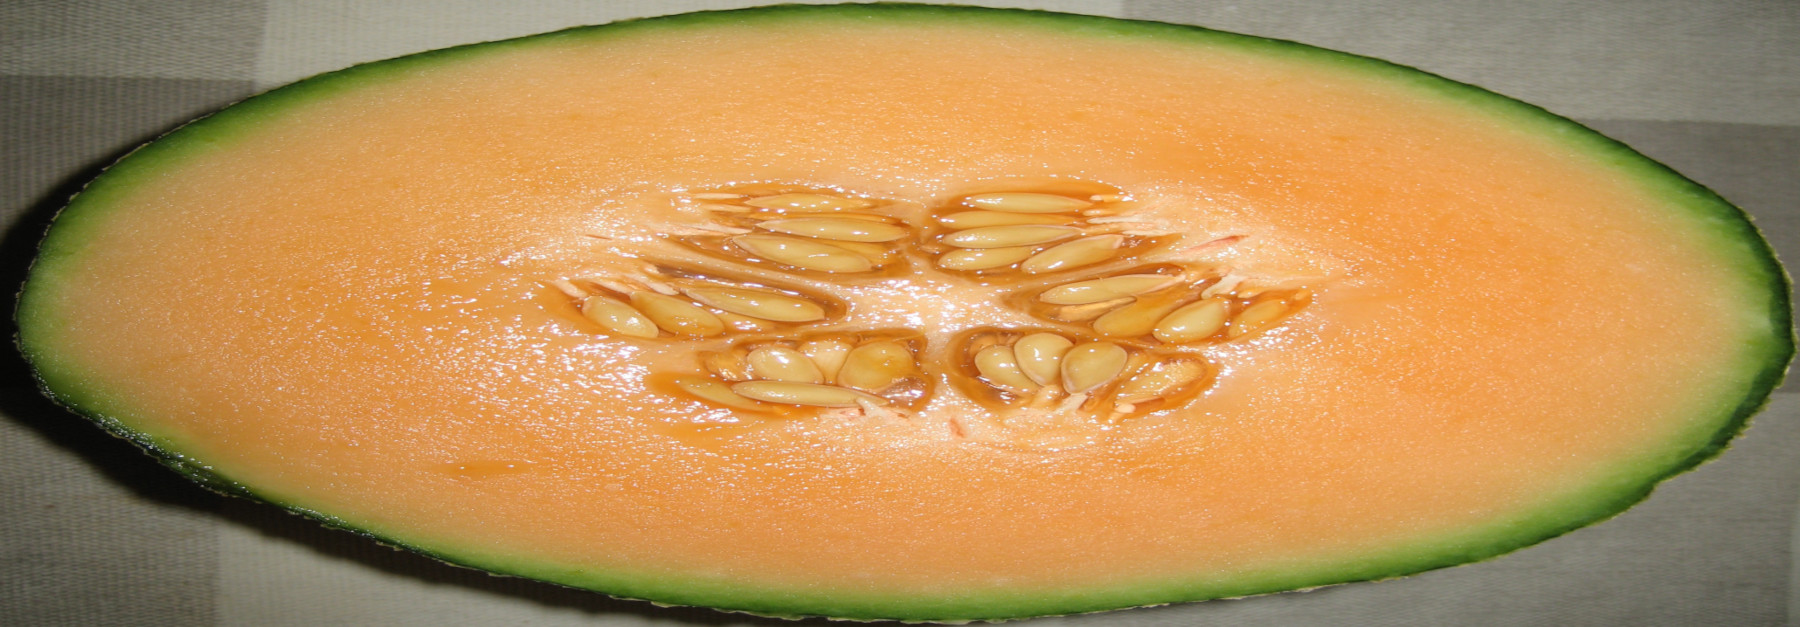
\includegraphics[width=5in]{images/cantaloupe}
\end{center}
\Instr{  Students should see that the cantaloupe is about 3 times wider than it is tall, giving the cross section a width to height ratio of 1:3. The cross section of an actual cantaloupe should have a width to height ratio of about 1:1 since the fruit is more or less spherical.}\wbvfill
\item Hand:
\begin{center}
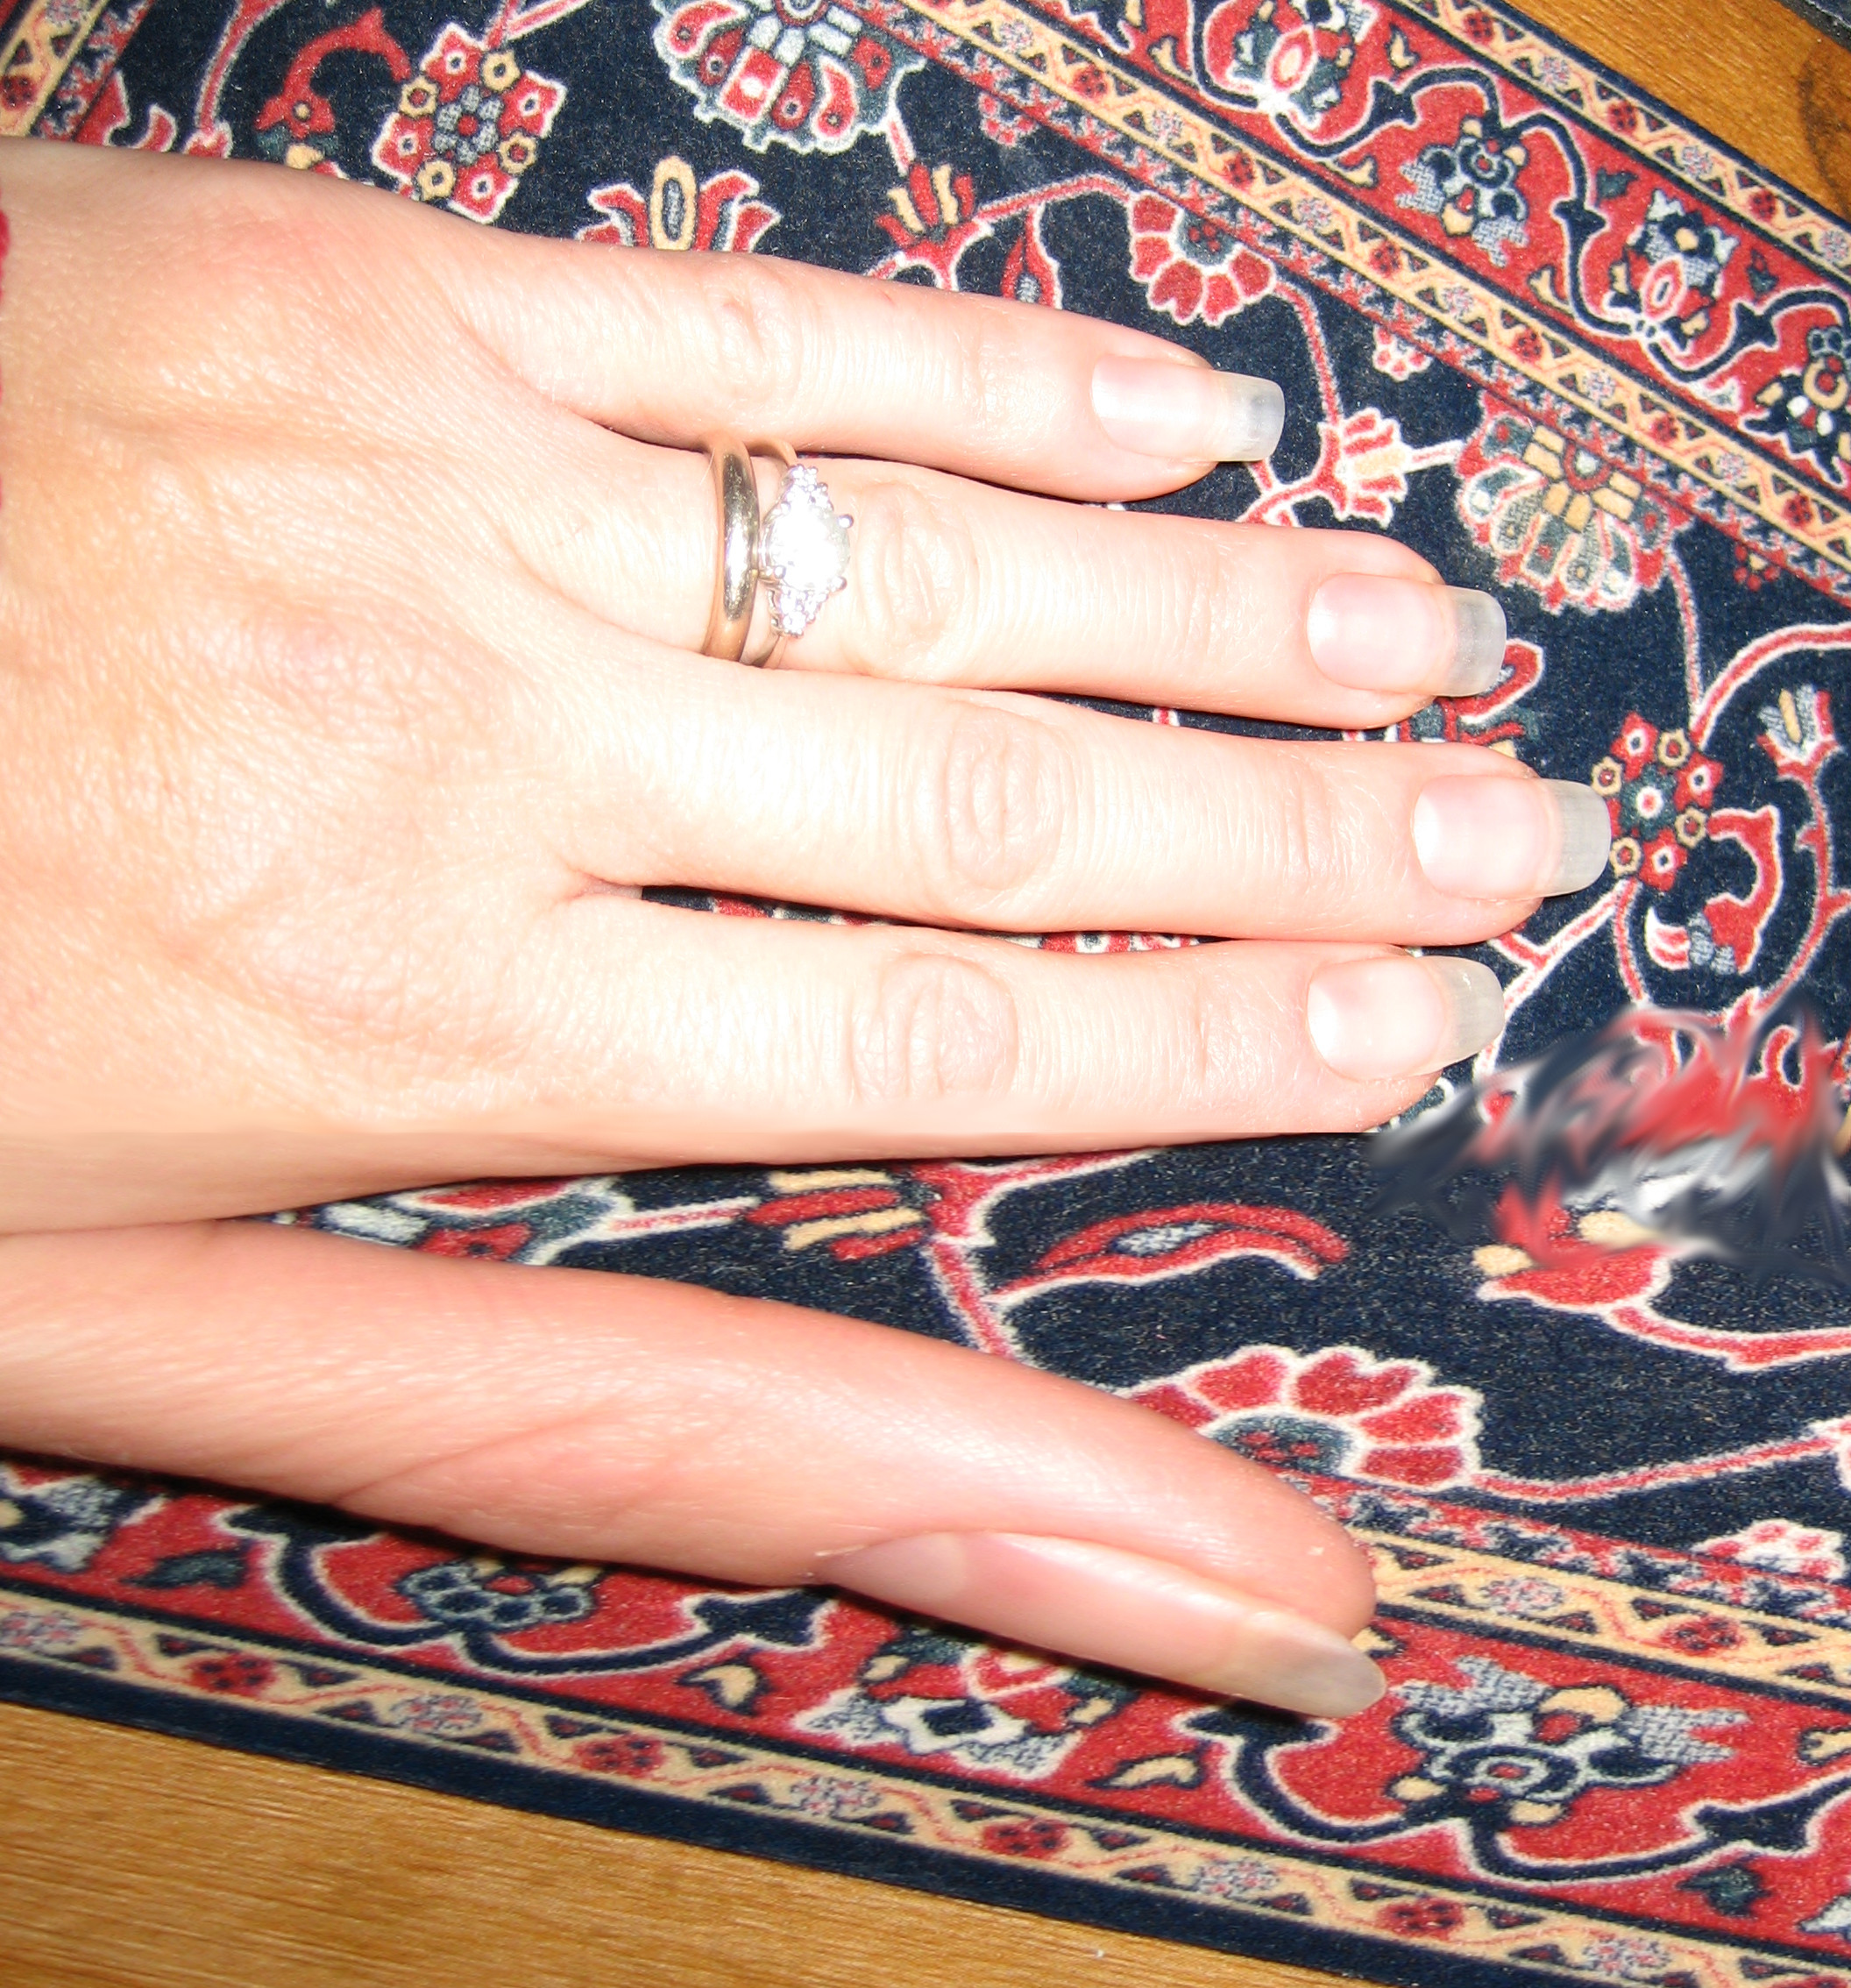
\includegraphics[width=2.5in]{images/thumb}
\end{center}
\Instr{  Students should see that the thumb is way out of proportion. Encourage them to use this phrase. If they don't do it themselves, have them measure their own fingers and thumbs to decide what a "normal" ratio of thumb length to pinky length or thumb length to ring finger length might be, and to compare it to the ratio in the photo.}\wbvfill
\end{enumerate}

\wbnewpage
\subsection{Exit Slip: Automobile, Cauliflower, and a Soccer Ball}
\begin{center}
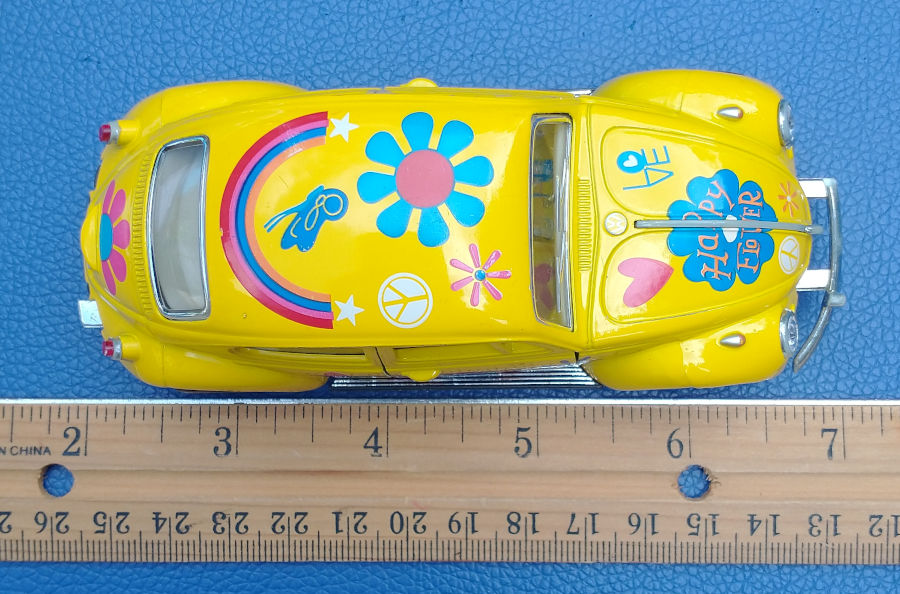
\includegraphics[height=1.7in]{images/lovebug} 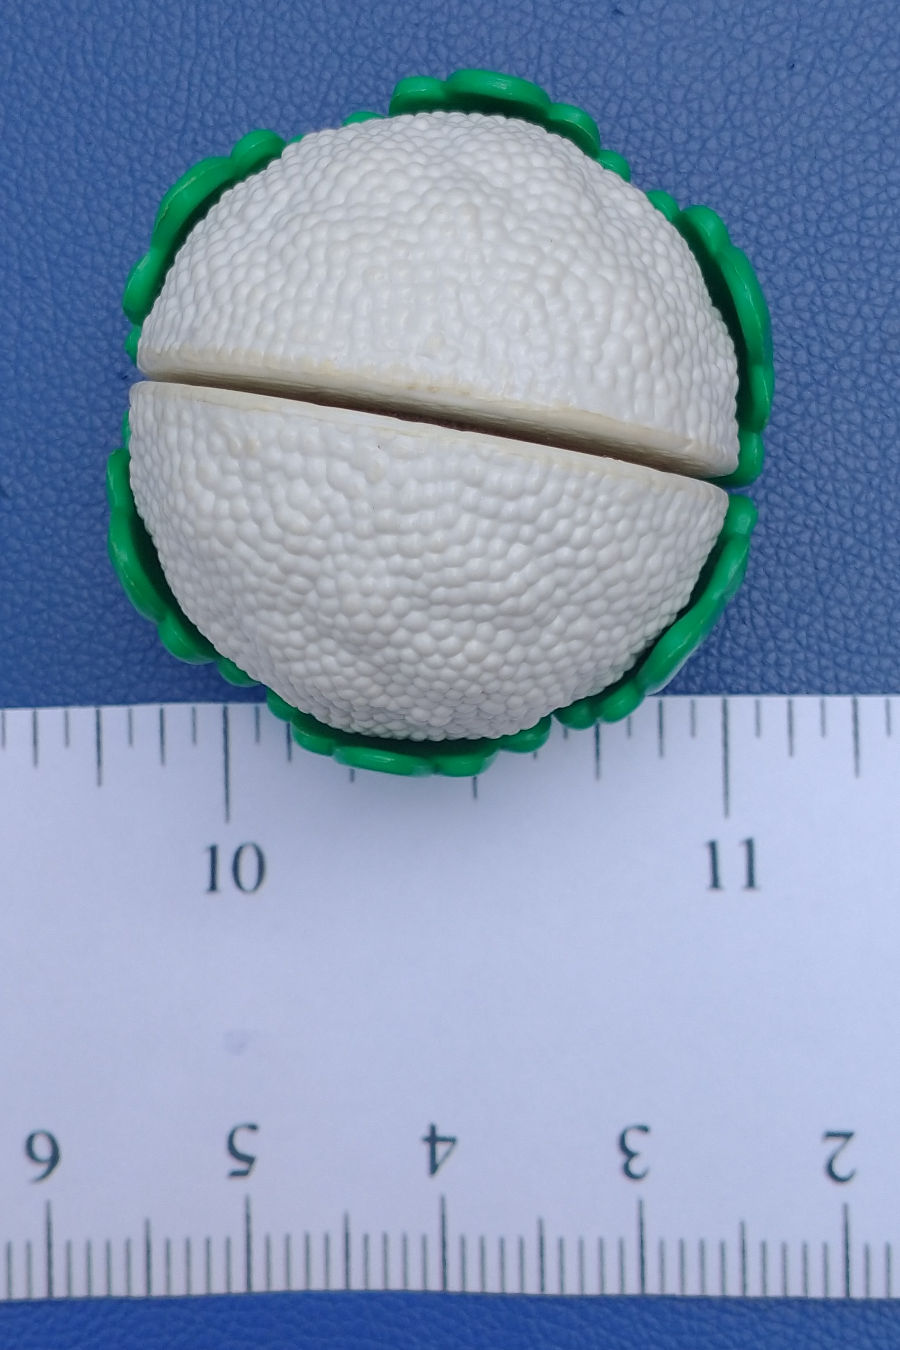
\includegraphics[height=1.7in]{images/cauliflower} 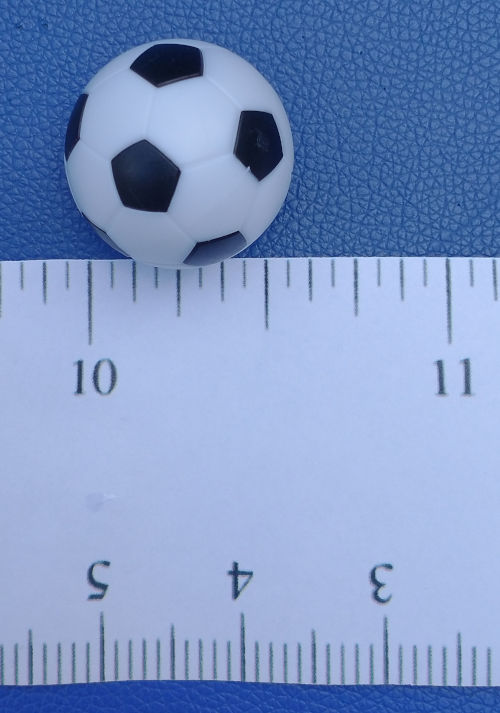
\includegraphics[height=1.7in]{images/soccerball}
\end{center}
\begin{enumerate}
\item Use the picture to measure the size of the model automobile, cauliflower, and soccer ball. \Instr{  5", 1.2", 0.6"}\wbvfill
\item Approximately what is the true (real-life) size of an automobile, head of cauliflower, and soccer ball? \Instr{  15', 7", 9"}\wbvfill
\item What are the scales of the
\begin{enumerate}
\item model automobile? \Instr{  1:36}\wbvfill
\item model cauliflower? \Instr{  1:5.8}\wbvfill
\item model soccer ball? \Instr{  1:15}\wbvfill
\end{enumerate}
\item Would it make sense to pair any of these objects in the same farmhouse diorama? Would the cauliflower and soccer ball look "right" next to each other? The cauliflower and automobile? The soccer ball and automobile? Explain. \Instr{  The cauliflower and soccer ball would not look right next to each other. In real-life, the soccer ball would be bigger, but the model soccer ball is actually smaller. To use the ratios to explain why they would not look right together, note that the soccer ball is shrunken almost three times as much as the cauliflower (since 15 is almost 3 times 5.8). The cauliflower and automobile would look even more out of proportion since the automobile is shrunken almost 6 times as much as the cauliflower (since 36 is more than 6 times 5.8). The cauliflower would look humongous next to the car. The only pair that might not look grossly out of proportion is the automobile and soccer ball. While the car is shrunken more than twice as much as the soccer ball, so the soccer ball will be too big in comparison, mathematically speaking it is rather out of proportion. However, it might not look entirely out of place. The wheel of the car looks to be about an inch in diameter, making the soccer ball (at 0.6") a good bit smaller than the wheel. That might be enough to make them look OK together.}\wbvfill\wbvfill
\end{enumerate}

\wbnewpage


\subsection{Entrance Activity: The Odditorium}
You're on a family vacation, and your parents get the idea to bring everyone to the nearby odditorium. You're not sure it will be any fun, but your parents are insistent and your sibling thinks it's a great idea. It turns out the things at the odditorium are truly odd. There's the world's smallest automobile, authentic shrunken heads, and sculptures made from recyclables. There's also this mannequin of the world's tallest person next to a young lady clearly enjoying the place. You spy the same young lady just outside the odditorium with this humongous marble.
\begin{center}
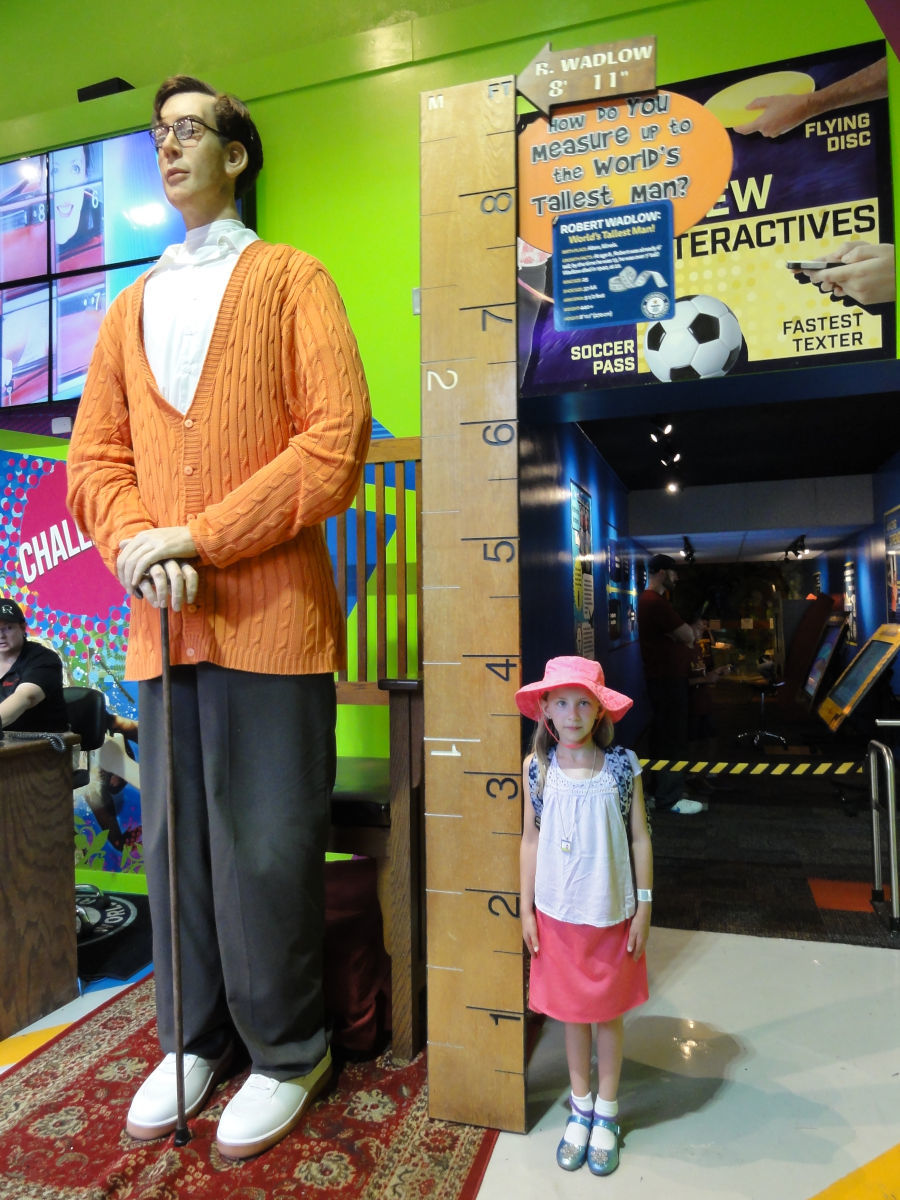
\includegraphics{images/OdditoriumTallMan} 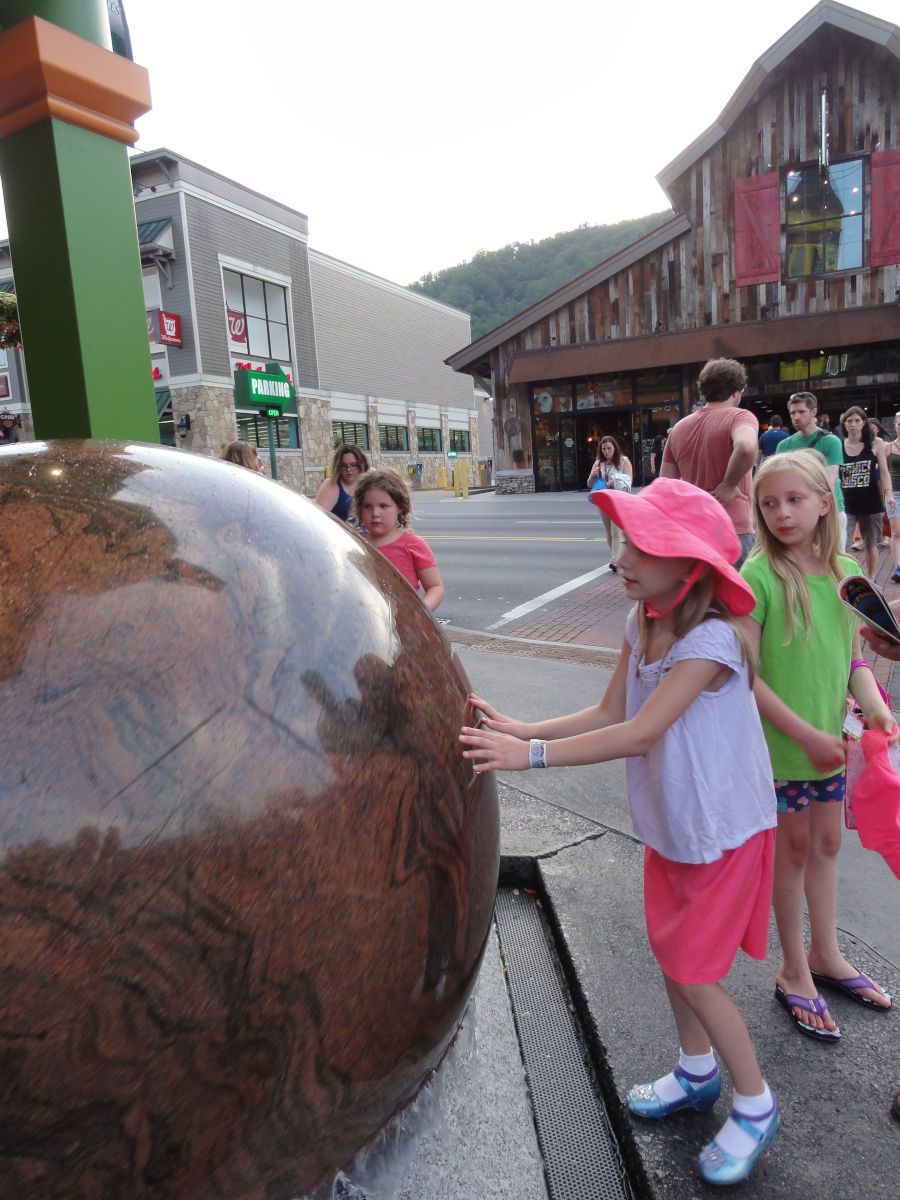
\includegraphics{images/OdditoriumSphereWithYouth}
\end{center}

\noindent Curiously, she is spinning the marble all by herself! The sign nearby notes that the sphere ``is floating on 1/254 inches of water and can easily be stopped and spun in another direction---try it!'' You think to yourself, ``that ball looks really heavy. Just how much weight is she pushing around?''

\begin{enumerate}
    \item Gather several stones, each one the size of a walnut or smaller. Put them somewhere so you won't forget to bring them to class!\wbvfill
    \item Make a guess as to the weight of the giant marble.\wbvfill
\end{enumerate}

\wbnewpage
\noindent Before starting this activity take a good look at the pictures from the entrance slip. Use them to estimate the diameter of the humongous marble. \Instr{  From the picture with the mannequin of the world's tallest person we can see the girl is almost exactly 4 feet tall to the top of her hat. The top of the marble is clearly higher than the top of the girl's head. What is not as obvious is that the ball is sunken into the sidewalk a substantial amount. It's hard to estimate exactly, but it is 6 or more inches making the diameter of the marble almost 5 feet.}

\subsection{Activity: Marble Weight Using Density}
The density of an object is the ratio of its mass to its volume. In this activity, we will determine the densities of the stones you brought to class and use that information to predict the weight of the giant marble at the odditorium.
\begin{enumerate}
    \item Choose one of the stones you brought to class and
    \begin{enumerate}
        \item use the scale to find its mass\wbvfill
        \item use the graduated cylinder to find its volume\wbvfill
        \item write down the density of the stone as a ratio. Use colon notation and integers on each side of the colon.\wbvfill
    \end{enumerate}
    \item Repeat for two of the other stones.
    \item Do any of the densities you calculated seem wrong, or did they all come out about the same?\wbvfill
    \item \label{enu:stonedensity}Pick one of the densities as an estimate of the density of the stones you brought in. Choose the density you think best matches the density of the marble in the picture.\wbvfill
    \item \label{enu:stonevolume}Using your estimate of the diameter of the giant marble, calculate its volume. The volume of a sphere is $V=\frac43\pi r^3$.\wbvfill
    \item Calculate the mass of the giant marble based on your answers to questions \ref{enu:stonedensity} and \ref{enu:stonevolume}. \wbvfill
\end{enumerate}

\wbnewpage
% New Section %%%%%%%%%%%%%%%%%%%%%%%%%%%%%%%%%%%%%%%%%%%%%%%%
\section{Project Choices}\label{sec:RatiosProjects}
%%%%%%%%%%%%%%%%%%%%%%%%%%%%%%%%%%%%%%%%%%%%%%%%%%%%%%%%%%%%%%

\begin{enumerate}
\item Unit Conversion
\begin{enumerate}
	\item\textbf{Paradox resolved} A 12"$\times$10" rectangular prismic foot bath is filled 3" deep using water from a 10' diameter circular pool (see photo). Knowing that water has been removed from the pool for use in the foot bath, logic would suggest that the level of water in the pool must decrease. The pool contains less water after all! However, the pool looks just as full after removing water as it did beforehand. What gives?
	\begin{center}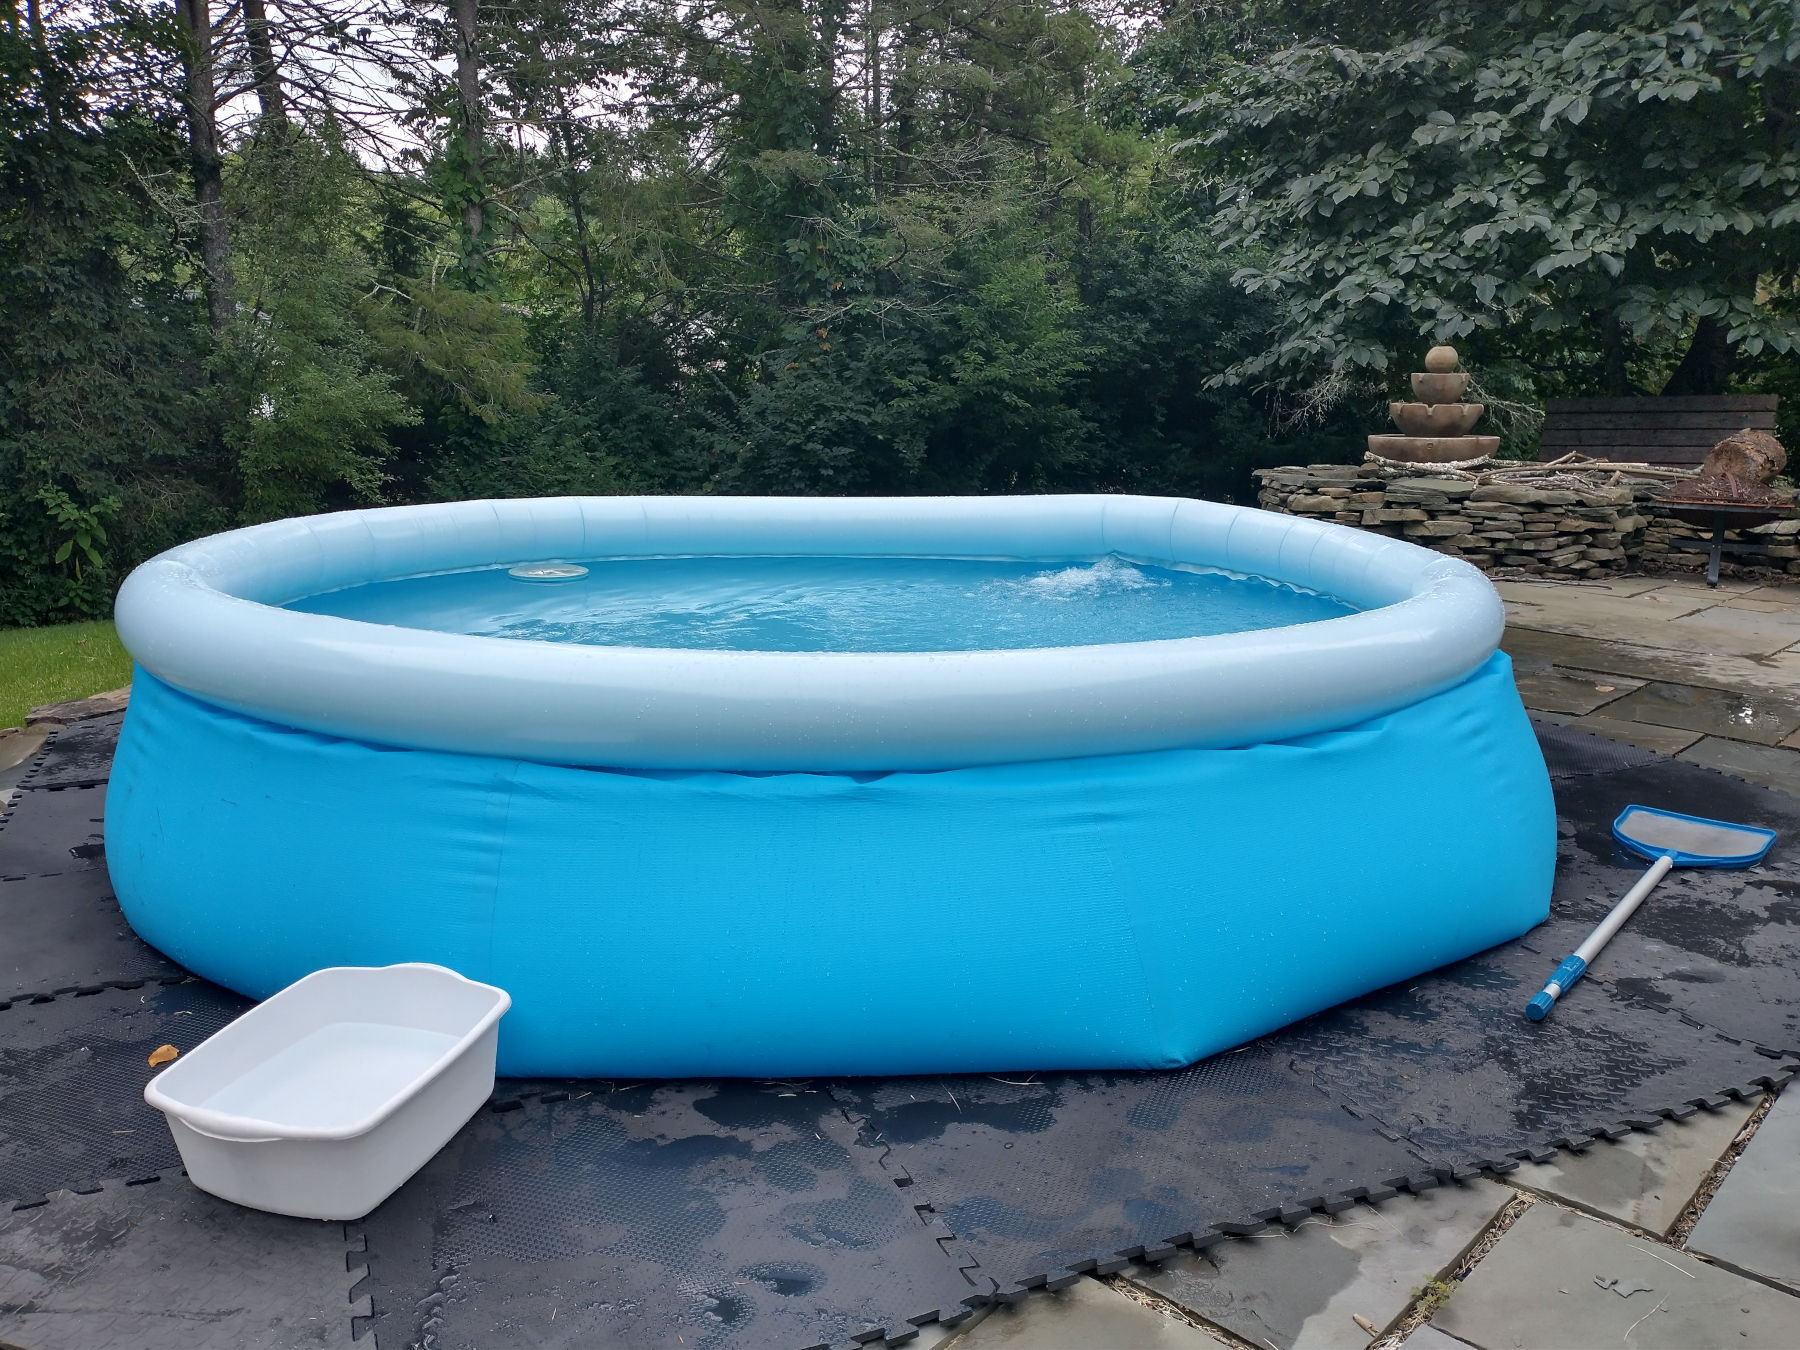
\includegraphics[width=3in]{images/pool}\end{center}
	\begin{enumerate}
		\item \label{en:footbath}Calculate the volume of water removed from the pool in cubic inches.
		\item \label{en:depthdecrease}A cylinder with diameter 10' and the same volume as that calculated in part \ref{en:footbath} has what height (in inches)? NOTE: The volume of a cylinder is $V=\pi r^2h$ where $r$ is the radius of the cylinder and $h$ is its height.
		\item Explain why the height calculated in part \ref{en:depthdecrease} is a good approximation of the amount the level in the pool must have decreased.
		\item How does this calculation resolve the paradox?
	\end{enumerate}
	\item\textbf{Lake Mead} Formed by the Hoover dam, Lake Mead is the largest reservoir in the United States. Much of the lake straddles the border between Nevada and Arizona, states that have been in a drought for over two decades. Due to record low levels in the lake in 2022, the Bureau of Reclamation mandated water usage cutbacks in both Nevada and Arizona. In Nevada, the cutback is $21,000$ $\text{acre}\cdot\text{feet}$. (As reported in \href{https://sites.imsa.edu/acronym/2022/05/22/the-drought-affecting-lake-mead/}{The Acronym} May 22, 2022)
	\begin{enumerate}
		\item \label{en:Mead-ft3}Convert $21,000$ $\text{acre}\cdot\text{feet}$ to cubic feet using the fact that one acre is $43,560$ square feet.
		\item Convert the volume from part \ref{en:Mead-ft3} into gallons using the estimate that 25 cubic feet equals 187 gallons.
		\item Does this seem like a large cutback? Explain.
	\end{enumerate}
\end{enumerate}

\item Ratios
\begin{enumerate}
\item Verbalize the similarities, differences, and connections between the concepts of ratios, fractions, and unit conversion.
\item Would this Rubik's cube look abnormally small, abnormally large, or just about right in this doll's hands? Explain in terms of ratios.
\begin{center}
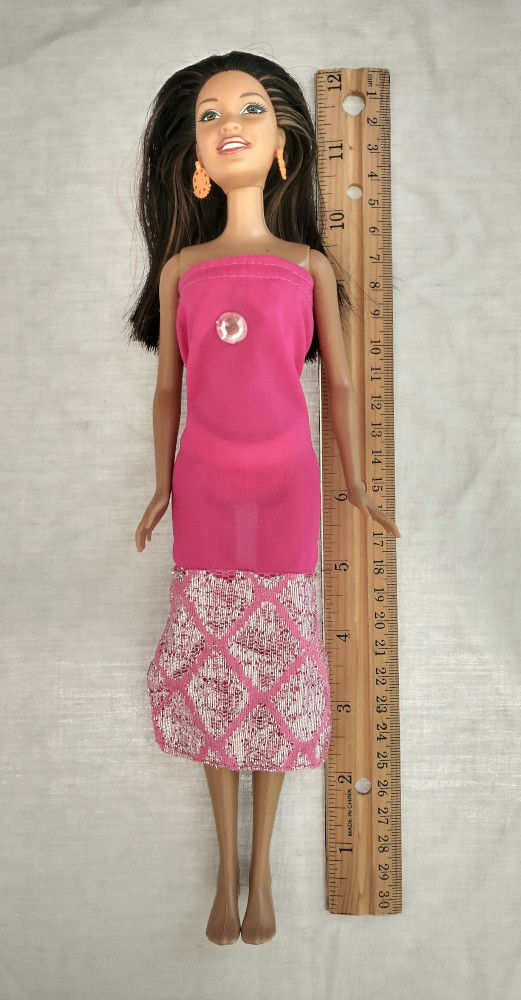
\includegraphics[height=3in]{images/doll} 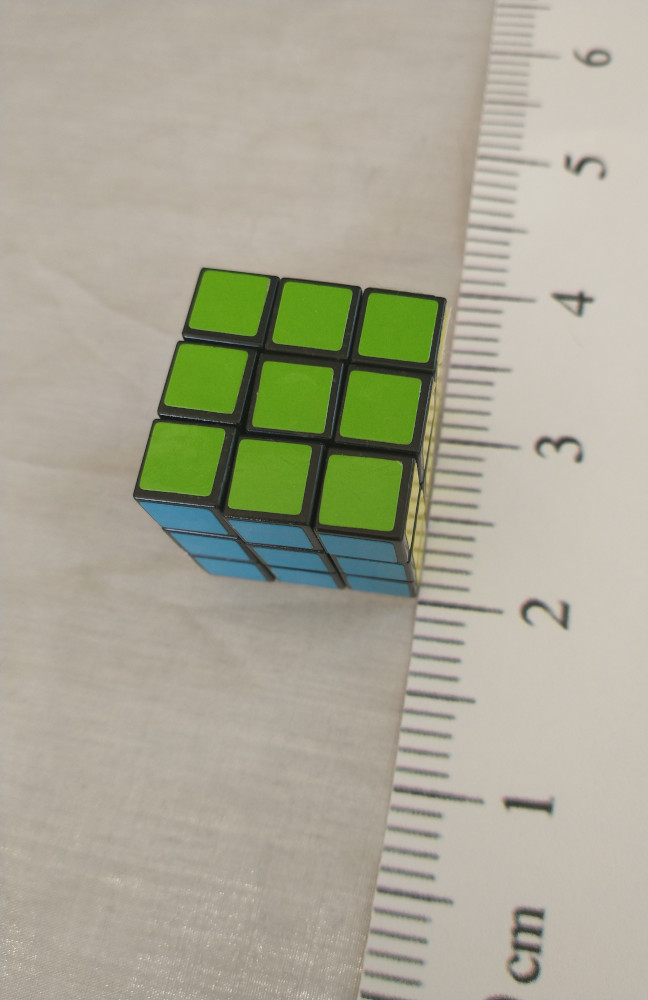
\includegraphics[height=3in]{images/RubiksCube}
\end{center}
\item In mixing pumpkin pie spice from individual spices, the ratio of cinnamon to ginger to cloves to nutmeg is 4:2:1:0.5. This means, for example, that you can mix 4 teaspoons cinnamon with 2 teaspoons ginger and 1 teaspoon cloves and a half teaspoon nutmeg to make 7.5 teaspoons of pumpkin pie spice.
\begin{enumerate}
\item How many tablespoons are 7.5 teaspoons? If you don't know the conversion between teaspoons and tablespoons, look it up! \Instr{  2.5 tablespoons}
\item How much of each ingredient should you use to make 6 tablespoons of pumpkin pie spice? \Instr{  6 is 12/5 times 2.5, so mathematically you should use, in teaspoons, 48/5 cinnamon, 24/5 ginger, 12/5 cloves, and 6/5 nutmeg.}
\item Is it practical to make 6 tablespoons of pumpkin pie spice using this recipe? \Instr{  No. Nobody has measuring spoons accurate to the nearest 1/5 of a teaspoon.}
\item What would be practical amounts of each spice to mix instead given that you need 6 tablespoons for your fall baking? \Instr{   Turning all the denominators of 5 into denominators of 6 (multiplying each by 5/6) yields practical amounts for each (8 tsp, 4 tsp, 2 tsp, and 1 tsp) but makes less than the requested 6 tablespoons. Simply tripling each of the original amounts would be practical and would make 7.5 tablespoons, of which you could use 6 and store the additional 1.5.}
\end{enumerate}
\end{enumerate}

\item Tile New Haven
The Area of New Haven The land area of New Haven, CT is 18.69 square miles (\href{https://www.census.gov/quickfacts/newhavencityconnecticut}{U.S. Census})

\begin{enumerate}
		\item Convert the area of New Haven into square feet. Note that square miles is written $\text{miles}^{2}$ (or $\text{miles}\times\text{miles}$) as a unit. Use the fact that $1\text{ mile}=5280\text{ feet}$. HINT: It's more than a million. \Instr{ Students will likely make the mistake of multiplying $18.69$ by $5280$ and calling it a day. The problem is that $18.69\text{ miles}^{2}\times\frac{5280\text{ feet}}{1\text{ mile}}=98,683\text{ miles feet}$, very strange units indeed! Only one of the miles cancels, just as $18.69x^{2}\times\frac{5280y}{x}=98683xy$.}
		\wbvfill
		\item A ceramic tile for a traditional subway tiling pattern is $2$ inches tall and $4$ inches wide. How many tiles does it take to cover one square foot?
		\wbvfill
		\item How many tiles would it take to cover the entire area of New Haven?
		\wbvfill
		\wbnewpage
		
		\item Convert the area covered by one letter size sheet of paper (which is $8.5$ inches wide and $11$ inches tall) into square feet.
		\wbvfill
		\item How many sheets of letter size paper would it take to cover New Haven? In other words, convert the area of New Haven from square feet into sheets of letter size paper.\Instr{ Using the given information, the student should arrive at 802,468,562 sheets.}
		\wbvfill
		
	\end{enumerate}


\end{enumerate}